% jakým způsobem jsem testovat, že co jsem udělal já funguje
\chapter{Ověření funkčnosti návrhu}
Tato kapitola se věnuje ověření funkčnosti návrhu a praktické implementace navrženého systému pro ovládání dopravníkové linky. Cílem provedených testů bylo potvrdit správnou činnost jednotlivých komponent i celkové integrace systému do prostředí typické dopravníkové linky a otestovat chování v reálném provozu.

\subsubsection{Způsob testování a prostředí}

Veškeré testování bylo provedeno v Brněnské hale společnosti Honeywell (viz. obrázek \ref{fig:BrnenskaHoneywellHala}). V té je rozmístěno několik různých plně funkčních dopravníkových systémů. Tato hala existuje primárně aby bylo možné ukázat potenciálním zákazníkům společnosti Honeywell jaké produkty firma nabízí, ale také velmi často slouží jako testovací prostředí pro inovace, jako je tento systém na ovládání dopravníků.

V době, kdy byla v hale testovaná funkčnost celého systému byla přibližně 80 metrů daleko v jiné části haly spuštěná jiná dopravníková linka, ale vzhledem k tomu, že vzdálenost dosahu WiFi signálu byla v rámci přijatelných mezí, lze předpokládat, že signál nebyl druhou linkou zarušený. Je ale potřebné zdůraznit, že charakteristiky šíření bezdrátového signálu a potenciální míra rušení v konkrétní lokalitě zákazníka se mohou významně lišit v závislosti na uspořádání dopravníků, přítomnosti překážek, hustotě instalovaných zařízení a dalších lokálních faktorech co by mohly rušit radiový signál.

\begin{figure}[hptb]
	\centering
	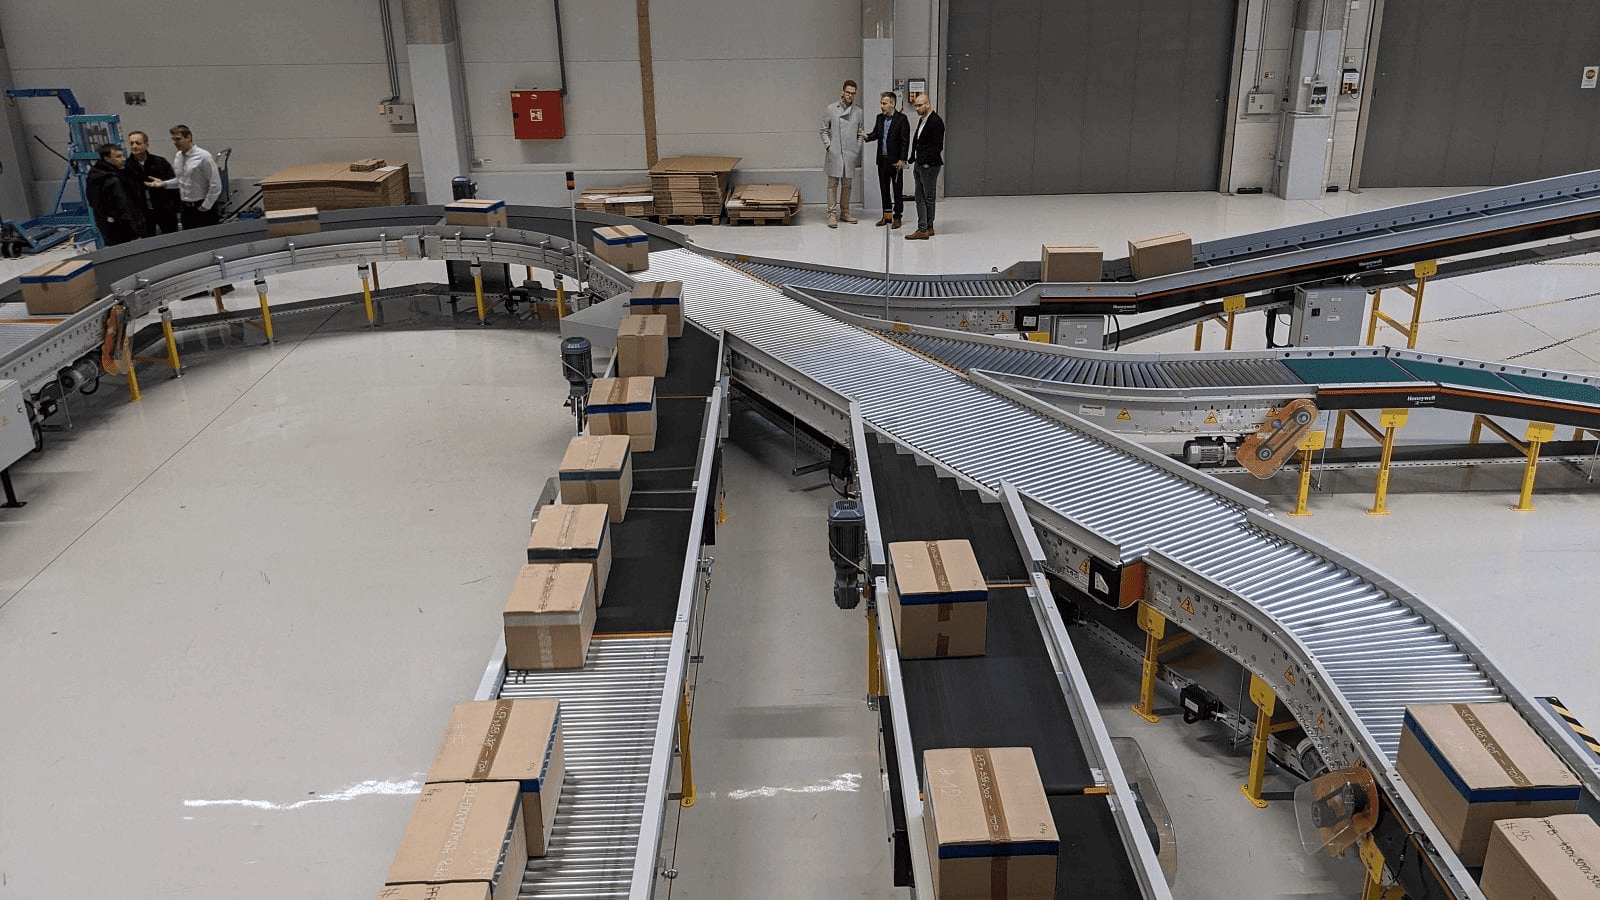
\includegraphics[width=1\linewidth]{images/BrnenskaHoneywellHala.png}
	\caption{Ukázka Brněnské haly pro testování dopravníků společnosti Honeywell \cite{HoneywellHala}}
	\label{fig:BrnenskaHoneywellHala}
\end{figure}

Způsob, jakým byl systém prvně otestován je skrz konfiguraci ovládacího panelu frekvenčního měniče podle instrukcí specifikovaných na stránce "/setup" dostupné uvnitř mobilní aplikace. Nejdříve byla rozpojena výkonová část frekvenčního měniče a poté byl nastavený. Po dokončení softwarové konfigurace byla deska připojena na digitální vstupy do ovládacího panelu frekvenčního měniče včetně stejnosměrného $24V$ napájení z výstupního napájecího portu ovládacího panelu.

Po otestování správnosti zapojení a konfigurace pomocí lokálního zapojení byla provedena zkouška s vypnutou výkonovou částí frekvenčního měniče a následně i se zapnutou výkonovou částí frekvenčního měniče, kde se dopravník začal pohybovat, jak bylo předpokládáno. Při uvádění dopravníku do provozu se zapnutou výkonovou částí je potřebné zajistit, aby v systému nebyla načtená hodnota aproximace rychlosti dopravníku jiná než 0. Zanedbání tohoto kroku vede k tomu, že bude systém ukazovat v mobilní aplikaci i na LCD displeji posunutou hodnotu rychlosti.

%%%%%%%%%%%%%%%%%%%%%%%%%%%%%%%%%%%%%%%%%%%%%%%%%%%%%%%%%%%%%%%%%%%%%%%%%%%%%%%%%%%%%%%%
\oldtext
%%%%%%%%%%%%%%%%%%%%%%%%%%%%%%%%%%%%%%%%%%%%%%%%%%%%%%%%%%%%%%%%%%%%%%%%%%%%%%%%%%%%%%%%

\section{Ověření funkčnosti lokálního ovládání}
% \purpose{Tady bych se chtěl zaměřit na to, jestli je možné dopravník ovládat přes tlačítka rovnou umístěná na desce.}

Funkčnost lokálního ovládání byla ověřena tím způsobem, že se nejdříve otestovalo, že je možné ovládat dopravník s vypnutou deskou a poté se deska připojila a znovu se testovalo jestli je možné dopravník ovládat s připojenou deskou, která je nastavená na lokální režim ovládání.

Při připojení systému na dopravník bez připojení napájecího kabelu bylo vidět, že LCD displej nefunguje a v mobilní aplikaci není dostupná předchozí IP adresu. Dopravník bylo stále možné ovládat, jelikož je deska plošných spojů provedena tím způsobem, že když není napájena, je ovládána lokálně.

Při připojení systému na dopravník s připojením napájecího kabelu se ihned spustil LCD displej a bylo vidět, že se vývojová deska snaží připojit na hotspot. Po připojení bylo možné vidět IP adresu vývojové desky i v mobilní aplikaci. Při nastavení přepínače na polohu ve kterém je deska lokálně ovládaná bylo stále možné ovládat dopravník pomocí tlačítek na schránce. Potvrdilo se tedy, že v tomto módu ovládání deska neposílá žádné napětí na sepnutí MOSFET transistorů co spínají relé a tak systém stále funguje plně analogově. Při tomto módu zapojení je ale dostupná informace o rychlosti dopravníku jak na LCD displeji tak i v mobilní aplikaci.

\section{Ověření funkčnosti mobilní aplikace}
%\purpose{Tady jenom potvrdím že mobilní aplikace opravdu funguje}

Po úspěšném otestování analogového ovládání desky bylo přistoupeno k testování mobilní aplikace. Mobilní aplikace se už částečně otestovala při předchozím testu, kdy bylo vidět, že pokud je vývojová deska přidaná se správnou IP adresou do aplikace, lze vidět rychlost a způsob ovládání dopravníku i pokud systém není přepnutý do dálkového ovládání.

Pro další testování byl systém přepnutý do stavu dálkového ovládání pomocí přepínače který je umístěný na schránce systému. Při přepnutí do stavu dálkového ovládání dopravník ihned začal zpomalovat, protože bylo přivedené napětí na MOSFET tranzistor, který ovládá relé pro přepínání mezi typy ovládání - rozpojil se tedy obvod, který přiváděl vysokou digitální hodnotu na vstup do ovládacího panelu, který dopravník udržoval v zapnutém stavu. Následně bylo potvrzeno, že dopravník lze ovládat pomocí mobilní aplikace, která úspěšně posílala GET požadavky na WebServer a tak bylo vidět že vývojová deska přepíná relé, které na desce plošných spojů spíná digitální vstupy ovládacího panelu.

Při přepnutí do dálkového stavu ovládání bylo také v mobilní aplikaci vidět, že se typ ovládání změnil na variantu "Remote".

\section{Ověření spolehlivosti dálkové komunikace}
%\purpose{Potvrdit že jsem schopný odejít na několik desítek metrů bez toho abych ztratil signál}

Při zapojení systému s dálkovým ovládáním bylo možné otestovat i vzdálenost komunikace, kterou je možné se systémem dosáhnout. Pro otestování dosažitelné vzdálenosti bylo zvoleno jít směrem dále od druhé spuštěné dopravníkové linky, aby bylo méně pravděpodobné, že se WiFi signál zaruší. V rámci testování byl také celý systém umístěn tak, aby byla z pozice mobilní aplikace viditelná anténa vycházející ze schránky. Tímto způsobem byl dosažen dosah WiFi komunikace kolem 35 metrů.

Tento dosah je přijatelný, protože dálkové ovládání bude mít nějvětší přínos například pokud budou mechanické zkoušky prováděny na dopravnících, které jsou instalované pod stropem skladové haly. V těchto případech se výška dopravníků může pohybovat kolem 10 metrů a tak je dosah 35 metrů dostatečný i pro tyto případy.

\section{Ověření funkčnosti zapojení více desek}
\purpose{Tady bych se rád zaměřil na nějaké testy, při kterých zkouším, jestli je opravdu možné ovládat víc desek zároveň.}

Pro otestování jsem nastavil a zapojil dvě desky podle návodu u dvou dopravníků několik metrů od sebe. Následně jsem testoval vzdálenost kde se mi podařilo si zachovat spojení s obouma deskami na X metrů. Tohle bylo znovu testované v Brněnské Honeywell hale. Při testování jsem sledoval jestli se dopravníky hýbou tím, že jsem si na dopravník položil testovací balík a u toho bylo vidět, jestli se při dané vzdálenosti hýbe anebo už ne.

\section{Posouzení z hlediska bezpečnosti}\label{sec:PosouzeniZHlediskaBezpecnosti}
\purpose{Tady bude nějaký moje zamyšlení nad bezpečností téhle desky. }

Ta deska už ze své podstaty má umožňovat ovládat dopravník na dálku a někdy i třeba hodinu - aby si sedly všechny součásti a tak bylo vidět, jestli je dopravník opravdu v pořádku za chodu. Tohle může být inherentně nebezpečná věc pokud by operátor přišel o spojení s deskou ve špatný okamžik a nemohl tak dopravník zastavit. Je možný, že by měla obsahovat nějakej test (třeba každou sekundu), jestli je otevřená aplikace na mobilu, ale to by kazilo user experience uživatelů, který dělají ty testy, protože oni musí při používání aplikace ještě psát informace o zkouškách do excelu. Pokud by se aplikace zavřela, tak přestane komunikovat s deskou a ta by pak chtěla ten dopravník vypnout. Tenhle bezpečnostní mechanismus tedy nemá smysl implementovat, protože by příliš kazil používání systému jako takového.

Myšlenku žádný takový mechanismus nevytvářet také podporuje fakt, že navržený systém přebírá bezpečnost z těch už nainstalovaných dopravníků. Dopravníky už při této fázi kontroly kvality mají kolem sebe E-STOP lanko a E-STOP tlačítka, které jsou nastavené aby dopravníku přikázali pohotovostní zastavení, jak vyžaduje bezpečnost na pracovišti.

V rámci bezpečnosti je také důležité správně vyškolit obsluhu systému pro bezpečné používání systému. Obsluha by měla například vědět, že je potřebné vypnout výkonovou část frekvenčního měniče pomocí nainstalovaného vypínače při veškeré manipulaci s ovládacím panelem. Obsluha by také měla vědět jak správně systém nastavit a jak řešit časté problémy - obě témata obsahuje mobilní aplikace na adresách Setup a Help.